\documentclass{article} % For LaTeX2e
\usepackage{nips15submit_e,times}
\usepackage{hyperref}
\usepackage{url}
\usepackage{graphicx}
\usepackage{subcaption}
\usepackage{amsthm}
\usepackage{algorithm}
\usepackage[noend]{algpseudocode}

\newcommand{\Expect}{{\rm I\kern-.3em E}}
\algdef{SE}[DOWHILE]{Do}{doWhile}{\algorithmicdo}[1]{\algorithmicwhile\ #1}

\usepackage{mathtools}

\DeclarePairedDelimiterX{\infdivx}[2]{(}{)}{%
  #1\;\delimsize\|\;#2%
}
\newcommand{\infdiv}{D\infdivx}
\DeclarePairedDelimiter{\norm}{\lVert}{\rVert}

\theoremstyle{definition}
\newtheorem{definition}{Definition}[section]
\newtheorem{theorem}{Theorem}[section]
\newtheorem{corollary}{Corollary}[theorem]
\newtheorem{lemma}[theorem]{Lemma}
\newtheorem{assumption}{Assumption}
%\documentstyle[nips14submit_09,times,art10]{article} % For LaTeX 2.09
\title{}
\author{}
\newcommand{\fix}{\marginpar{FIX}}
\newcommand{\new}{\marginpar{NEW}}
\nipsfinalcopy % Uncomment for camera-ready version
\begin{document}

\maketitle

\begin{abstract}
We seek to contribute:\\
1) A clear understanding of Partial Observability as it relates to
state, agent, and task.\\
2) A measure of the degree to which a domain is partially observable.\\
3) A way to quantify the deficiency of a given state representation.\\
\end{abstract}

\section{Definitions}
The following definitions assume a fixed state representation. If we
have the ability to manipulate the state representation, the same
stochastic process can be Markov or non-Markov.

\begin{definition}[Markov Property]
A stochastic process has the Markov property if the conditional
probability distribution of future states of the process (conditional
on both past and present states) depends only upon the present state,
not on the sequence of events that preceded it.
\[
P(s_{n+1} | s_{n}, s_{n-1}, \dots, s_{1}) = P(s_{n+1} | s_{n})
\]
\end{definition}

\begin{definition}[k-order Markov Chain]
A Markov chain of order $k$ has the property that:
\[
P(s_{n+1} | s_{n}, s_{n-1}, \dots, s_{1}) = P(s_{n+1} | s_{n}, \dots, s_{n-(k-1)})
\]
The future state $s_{n+1}$ depends on the past $k$ states. Remembering
$k$ states restores the Markov property and a larger memory grants no
further predictive power.
\end{definition}

\begin{definition}[Entropy]
\label{def:entropy}
The entropy of a discrete random variable $X$ with alphabet $\mathcal{X}$ is
defined by:
\[
H(X) = -\sum_{x\in \mathcal{X}} p(x) \log p(x)
\]
\end{definition}

\begin{definition}[Mutual Information]
The mutual information between two random variables $I(X;Y)$ is the
reduction of uncertainty of $X$ due to knowledge of $Y$:
\[
I(X;Y) = \sum_{x,y} p(x,y) \log \frac{p(x|y)}{p(x)} = H(X) - H(X|Y)
\]
\end{definition}

\section{Introduction}
The relationship between state, observation, reward, and task, is
nuanced and deserves careful attention. Much of the discussion below
stems from the careful analysis of state and observability presented
in \cite{McCallum96}.

At a high level, reinforcement learning begins with an idea of a task
that a learning agent should perform. Two example tasks which we will
revisit are Texas Hold'em and autonomous driving. In the first task,
one might desire the agent to learn to play the card game Texas
Hold'em, and be capable of competing against other players. In
autonomous driving the agent must learn how to safely control the
vehicle in the presence of other drivers and navigate to a
destination.

More than general concept of desired functionality is required. A
reinforcement learning practitioner must provide a state or
observation space, an action space, and a reward space.

A state space $\mathcal{S}$ encodes information about the state of the
world. Useful state spaces transmit information that is relevant to
performing the desired task. Additionally, valid state spaces are
Markov, meaning that the distribution over next states is
conditionally independent of the history of past states. In this
paper, we additionally require state spaces to encode all of the
necessary information to perform the task (see definition
\ref{def:takRelState}). In contrast, an observation space
$\mathcal{O}$ encodes incomplete or noisy information and is not
required to be markov. Knowledge of the task is often sufficient to
understand if the available perceptual information is complete enough
to be considered a state or merely an observation. For example, in the
autonomous driving task, the vehicle's sensors provide information
about the physical world, and these sensations constitute the
observation space of the task. Due to the complexity of the real world
and the limited perceptions of present-day hardware, it's safe to
presume that the available information would encode an observation
space. In some tasks, the state/observation space is predefined and
immutable, but in other tasks like autonomous driving, it's possible
to modify the perceptual space, perhaps by adding additional sensors.

These ideas are alternatively understood as Markov Decision Process
(MDP) and a Partially Observable Markov Decision Process (POMDP): A
MDP is a 5-tuple $(\mathcal{S}, \mathcal{A}, \mathcal{P}, \mathcal{R},
\gamma)$, which represents an instantiation of a fully observed
learning task in which the perceptions of the agent are states
$\mathcal{S}$ (e.g. markov and complete). $\mathcal{A}$ defines the
action space, $\mathcal{P}$ is a transition function which describes
the dynamics of state change, $\mathcal{R}$ is a reward function
mapping states to scalar rewards, and $\gamma$ is a discount factor
describing the importance of immediate versus distant reward. A POMDP
is a 6-tuple $(\mathcal{S}, \mathcal{A}, \mathcal{P}, \mathcal{R},
\mathcal{O}, \gamma)$. The true states of the environment are hidden
from the agent. Instead, the agent perceives only observations
$\mathcal{O}$. MDPs and POMDPs are convenient formalisms, but only
approximate many tasks. For example, the task of autonomous driving
features an unknown (and perhaps unknowable) transition function and
state space.

In practice, a reinforcement learning task $\mathcal{Z}$ is defined by
a reward function $\mathcal{R}$, an action space $\mathcal{A}$, an
observation space $\mathcal{O}$ or state space $\mathcal{S}$, and a
discount factor $\gamma$. An optimal policy for a given task $\pi^*:
\mathcal{O} \rightarrow \mathcal{A}$ is a mapping from observation to
action that maximizes the expected returns $\mathcal{J} =
\Expect_{\pi^*}[\sum_{t} \gamma^t r_t]$.

Since much of this article is concerned with understanding
and characterizing state representations, we first define two
properties of observation spaces.

\begin{definition}[Policy-Markov]
An observation space $\mathcal{O}$ is \textit{Policy-Markov} if the set
of memory-free optimal policies over $\mathcal{O}$ is equivalent to
the set of memory-based optimal policies over $\mathcal{O}$. In other
words, a policy-markov observation space is one in which the optimal
policy does not change if additional memory is provided. $\mathcal{O}$
is policy-markov if and only if for all sequences of observations:
\[
\pi^*(o_{t}, o_{t-1}, \dots, o_{1}) = \pi^*(o_{t})
\]
The standard definition of the Markov property is concerned only with
predicting the next state. While the ability to predict future state
is useful for creating a model of the environment, the more pratical
concern is that of learning an optimal policy.
\end{definition}

Another useful definition allows two observation spaces to be compared
in terms of optimal policies:

\begin{definition}[Optimally-Equivalent]
A observation space $\mathcal{O}$ is said to be
\textit{Optimally-equivalent} to another observation space
$\mathcal{U}$ if the space of optimal policies in $\mathcal{O}$ is
equivalent to the space of optimal policies in $\mathcal{U}$. In other
words, two observations spaces are said to be optimally equivalent if
and only if they include the same optimal policies.
\end{definition}

For any task, let us consider the performance of the omnipotent
agent. This imaginary agent has access to the true state of the entire
universe down to the locations of every particle in every galaxy. As a
result, the omnipotent agent, when presented with a task, will always
ignore the task-defined observations, instead preferring to rely on
its own knowledge of state. Formally it is operating in a different
task $\mathring{\mathcal{Z}}$, where the task-defined observations
have been replaced with the agent's knowledge of true state
$\mathcal{S}$. This new state space includes an optimal policy
$\mathring{\pi}^*: \mathcal{S} \rightarrow \mathcal{A}$ that is at
least as good as the optimal policy in the observation space:
$\mathring{\mathcal{J}}^{\mathring{\pi}^*} \ge \mathcal{J}^{\pi^*}$.

For any given task, the omnipotent agent likely only requires a subset
of the true state $\mathcal{S}_\mathcal{Z} \subseteq \mathcal{S}$ in
order to learn an optimal policy. Subset $\mathcal{S}_\mathcal{Z}$
captures all the \textit{task-relevant-state} and ignores knowledge
that is irrelevant to the task at hand. For task $\mathcal{Z}$, the
class of optimal policies defined over $\mathcal{S}_\mathcal{Z}$ is
equivalent to the class of optimal policies over $\mathcal{S}$. In
Texas Hold'em, the task-relevant-state includes knowledge of the cards
in other players' hands, knowledge of the order of cards in the deck,
and emotional states of the other players, but does not include
inconsequential information such as the temperature on top of Mount
Everest. While the notion of an omnipotent agent is purely
theoretical, task-relevant-states are well defined for some
single-player games like Solitaire, in which the order of the cards in
the deck as well as the face-up cards provide a task-relevant-state.

\begin{definition}[Task-Relevant-State]
\label{def:taskRelState}
A task-relevant-state representation $\mathcal{S}_\mathcal{Z}$ is a
subset of world-state $\mathcal{S}$ that is both Policy-Markov and
optimally-equivalent to $\mathcal{S}$. The ideal task-relevant-state
representation is the smallest possible subset of $\mathcal{S}$ that
fulfills these conditions. Task-relevant-state is exactly the state
representation desired in a Markov Decision Process as it allows a
reactive, memory-free agent to learn an optimal policy that performs
as well as if the agent was omnipotent. In practice however, many
tasks lack a well defined or computable task-relevant-state.
\end{definition}

However, the complexity (and fun) of many tasks stems from hidden
state. Texas Hold'em, like Solitaire, is intended to be played with
partial information. Every task must define an observation space - in
the case of Texas Hold'em, a reasonable observation space is the
player's cards and community cards. In autonomous driving, the
observations are the perceptions from the laser range-finders,
cameras, and other sensory equipment. While in the best case, the
agent's observations may provide the task-relevant-state, in general,
the observation space is unlikely to be optimally-equivalent to the
task-relevant-state space. However, the degree of suboptimality
depends on the relationship between the task-relevant-state and the
observation space.

In the worst case, which we denote
\textit{irreversible-information-loss}, observations may irreversibly
lose important state information: the Texas Hold'em agent can't
perceive the community cards, or the autonomous vehicle's range-finder
is broken. In this case, even maintaining a full memory over past
observations will not help recover the missing information.

In the more benign case of \textit{memory-reversible-loss}, the
observation space is non-Policy-Markov, meaning that a memory of past
observations yields better optimal policies. In Texas Hold'em, this
could involve remembering that another player tends to bluff often and
using this fact to call his raise. An observation space may feature a
mix of irreversible information loss and memory reversible
loss. Section ? presents a method for quantifying the amount of
reversible and irreversible information loss.

\section{Partial Observability}
In the context of reinforcement learning, partial observability
describes the category of agent-environment interactions in which an
agent's perceptions do not provide complete information about the
task-relevant-state of the environment. This problem is also known as
\textit{incomplete perception}, \textit{perceptual aliasing}, or
simply \textit{hidden state}.

Information loss (memory-reversible or otherwise) is the effect of
partial observability. The means of information loss differs. One
cause of partial observability is perceptual aliasing, in which
multiple task-relevant-states all map to the same observation. Another
cause is sensor noise, in which a single task-relevant-state is
observed differently each time it is revisited. Figure
\ref{fig:functions} illustrates these cases.

\begin{figure}[htp]
\centering
\begin{subfigure}{.3\textwidth}
  \centering
  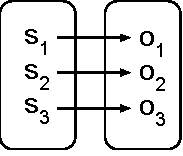
\includegraphics[width=.6\linewidth]{figures/bijection}
  \caption{Fully Observed}
  \label{fig:bijection}
\end{subfigure}
\begin{subfigure}{.3\textwidth}
  \centering
  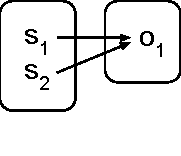
\includegraphics[width=.6\linewidth]{figures/state-aliasing}
  \caption{State Aliasing}
  \label{fig:state-aliasing}
\end{subfigure}
\begin{subfigure}{.3\textwidth}
  \centering
  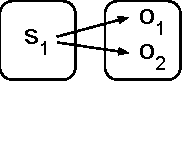
\includegraphics[width=.6\linewidth]{figures/noisy-perception}
  \caption{Noisy Perceptions}
  \label{fig:noisy-perception}
\end{subfigure}
\caption{A fully observed environment features an injective mapping
  from task-relevant-states to observations. Partial observability
  indicates the degree to which this injection is invalid. Two sources
  of partial observability are state aliasing, the degree to which the
  observation function is non-injective, and noisy perceptions, the
  degree to which the observation function is not a valid function.}
\label{fig:functions}
\end{figure}

\begin{definition}[Partial-Observability]
A task is partially observed if there is a loss of information between
the task-relevant-state representation and the task-defined
observations. We identify three tests for partial observability:
\begin{enumerate}
\item Assuming access to the task-relevant-state representation: A
  task is partially observable if and only if the mapping from
  task-relevant-states to observations is not one-to-one.
\item Assuming access to a omnipotent optimal policy: A task is
  partially observable if the omnipotent optimal policy
  $\mathring{\pi}^*$ performs better than an optimal policy $\pi^*$
  learned over the observation space.
\item Assuming access to neither: A task is partially observable if it
  is non-Policy-Markov.
\end{enumerate}
\end{definition}

\section{An Information-Theoretic View of Partial Observability}
One way to understand the partial observability of a task is to
quantify the amount of information the observations provide about the
task-relevant-states. Let us assume we have access to the true
environment state which generates each observation. Let $S$ be a
random variable over the domain of all possible states, and $O$ be a
random variable over all possible observations. The mutual information
$I(S;O)$ computes the reduction in uncertainty of the true environment
states $S$ resulting from knowledge of the observations $O$:

\[
I(S;O) = \sum_{s,o \in S \times O} p(s,o) \log \frac{p(s|o)}{p(s)} = H(S) - H(S|O)
\]

If the mapping from task-relevant-states to observations is
one-to-one, the mutual information $I(S;O)$ will equal $H(S)$, and the
agent's interaction with the environment is said to be fully observed.

\section{Using a History of Observations}
A natural technique to deal with partial observability is to augment
the agent's state representation to include a history of
observations. This strategy helps to address state aliasing by using
the observation history to disambiguate aliased states. In the case of
noisy observations, a history could be used to counteract noise, for
example by computing an average. However, the size of the state space
grows exponentially as a function of history length, so in practice it
is rarely feasible to maintain extensive history.

\begin{definition}[k-th Order Mutual Information]
Let $\textbf{O}^k$ be a random variable over the domain of all
k-length observation sequences $\textbf{o}^k = (o_t, o_{t-1}, \dots,
o_{t-(k-1)})$. We define the $k$-th order mutual information between
$k$-length observation histories and true states as follows:

\[
I(S;\textbf{O}^k) = \sum_{s,\textbf{o}^k \in S \times \textbf{O}^k} p(s_t,\textbf{o}^k) \log \frac{p(s|\textbf{o}^k)}{p(s)}
\]
\end{definition}

The growth of $I(S;\textbf{O}^k)$ as a function of $k$ reveals the
predictive power gained by leveraging additional history. Even
maintaining a full history cannot guarantee full observability in all
cases: in an extreme case where all states are mapped to the state
observation, even a full history is no help in predicting the next
state.

\section{Atari Games}
The state of an Atari game is fully specified by the 1024-bits of
console RAM. The Atari environment defines an observation function
$O(o|s)$ that maps RAM states to observed screens. This true state is
invisible to humans, who instead see the $160 \times 210 \times 3$
dimensional screen. Fortunately, the Arcade Learning Environment
provides access to both the RAM states and observed Atari screens.

A single Atari game screen often does not contain enough information
to disambiguate important aspects of state. Two examples: in the game
of Breakout, a single frame is sufficient to locate the position, but
not velocity, of the ball, which is necessary in order to correctly
position the paddle. Similarly, the player and opponent bullets in
Space Invaders look identical, so the only way to tell if a bullet is
approaching your ship or leaving it is to look at more than one
screen.

\subsection{Atari RAM Entropy}
We expect the RAM-entropy of will differ on a game-to-game
basis. There are several problems applying the standard definition of
entropy (Def \ref{def:entropy}) to Atari RAM-states:

\subsection{Stationary State Distribution}
In order to compute entropy, a distribution over RAM-states is
required. Atari does not provide access to the true distribution over
RAM-states, but instead allows sampling from this distribution in the
form of playing the game and recording the encountered
RAM-states. From any set of recorded RAM-states it is possible to
construct a distribution, but the constructed distribution may not
resemble the game's true distribution over RAM-states. In particular,
two questions arise: 1) What policy should be used to sample
RAM-states and 2) How many samples are necessary to ensure the
constructed distribution closely resembles the true distribution?
Before addressing these questions, let us define several
preliminaries:

\begin{definition}[Ergodic MDP]
An MDP $\mathcal{M}$ is ergodic if the Markov chain induced by any
policy is ergodic. An ergodic MDP is an MDP where every state can be
accessed in a finite number of steps from any other state.
\end{definition}

\begin{definition}[Episodic MDP]
An episodic MDP is an MDP with a terminal state that is accessible
from any state.
\end{definition}

\begin{definition}[Stationary State Distribution of Ergodic MDP]
\label{def:ssd}
An ergodic MDP has a stationary distribution $d^{\pi}(s)$ with the property:
\[
d^\pi(s) = \sum_{s' \in S} d^\pi(s')\mathcal{P}_{s',s}
\]
\end{definition}

Atari games are episodic MDPs with deterministic transitions. Formally,
episodic MDPs can never be ergodic since terminal states never
transition to any other state. However, it is possible to convert an
episodic MDP into an ergodic MDP by constructing an equivalent MDP
with each terminal state having a single action that transitions the
agent to the starting state.\footnote{The transition from the terminal to
starting state should have a discount factor of zero in order to
maintain equivalence of optimal values \cite{VanHasselt11}.}

Thus, playing multiple episodes of a given game under a fixed policy
$\pi$ is sufficient to define an ergodic MDP, and by definition
\ref{def:ssd}, for any fixed policy $\pi$, the Markov chain induced by
$\pi$ should have a stationary state distribution $d^\pi_\infty$. The
\textit{mixing time} of the Markov chain is the minimum amount of time
$t$ needed to ensure that $d^\pi_t$, the state distribution
constructed after $t$-steps, is epsilon close to the true stationary
state distribution $d^\pi_\infty$ (e.g. the distribution that would be
constructed after an infinite number of samples).

\begin{definition}[Mixing Time]
\label{def:ssd}
The mixing time $t_{\mathrm{mix}}(\epsilon)$ of an ergodic MDP is given by:
\begin{align*}
t_{\mathrm{mix}}(\epsilon) & = \min_t \norm{d^\pi_t - d^\pi_\infty}_{TV} \le \epsilon \\
& = \tfrac{1}{2}\sum_{s \in S} |d^\pi_t(s) - d^\pi_\infty(s) | \le \epsilon
\end{align*}
where $\norm{\cdot}_{TV}$ indicates the total variation distance.
\end{definition}

In general, it's hard to estimate mixing time...

In general, the distribution over visited states is a function of the
policy.



\begin{algorithm}
\caption{Dataset Collection}
\label{ram-ent}
\begin{algorithmic}
\State Given: Policy $\pi$, Error Bound $\epsilon$
\State $\mathcal{D} \gets \{\emptyset\}$ \Comment{$\mathcal{D}$ is the collection of all trajectories}
\Do
\State $\mathcal{D} \gets \mathcal{D}\ \cup \ $PlayEpisode$(\pi)$
\State $d^\pi_t \gets \ $ComputeStationaryStateDistribution($\mathcal{D}$)
\State $t\gets t+1$
\doWhile{$\norm{d^\pi_t - d^\pi_\infty}_{TV} > \epsilon$} \Comment{Wait until the state distribution converges}
\State \Return $d^\pi_t$
\end{algorithmic}
\end{algorithm}

\begin{definition}[Observability]
Assuming access to the true state distribution $S$ of an environment
as well as the observation distribution $O$, the observability
$\mathcal{O}$ of the environment is given by conditional entropy of
the true states given the observations, divided by the entropy of the
states.
\[
\mathcal{O} = 1 - \frac{H(S|O)}{H(S)}
\]
The observability quantifies how much information the observations
possess about the true environment state. Observability is always
between zero and one: an observability of zero indicates the
observations are no help in understanding the environment's state. An
observability of one implies the observations fully determine the true
state. Observability measure the degree of bijectivity in an
environment's mapping from states to observations.
\end{definition}


\section{Half Baked Ideas}
The following sections contain intuitions that may have some promise
but are poorly grounded.

\section{Sub-optimality induced by partial observability}
Partial observability causes agents to learn sub-optimal policies. The
degree of partial observability inherent in an environment bounds the
performance of an optimal policy learned over observations $\pi_O^*$
compared to the optimal policy learned over true states $\pi_S^*$:
\[
\textrm{sub-optimality} \propto \sum_{s\in S} D_{KL}\big(\pi_O^*(O(s))\ ||\ \pi_S^*(s)\big)
\]

\bibliographystyle{unsrt}
\bibliography{partialobs}
\end{document}
